%%%%%%%%%%%%%%%%%%%%%%%%%%%%%%%%%%%%%%%%%%%%%%%%%%
% Part: Introduction
% Filename: intro.tex
% Created: September 9, 2017
% Author: Adam Wright
%%%%%%%%%%%%%%%%%%%%%%%%%%%%%%%%%%%%%%%%%%%%%%%%%%


%%%%%%%%%%%%%%%%%%%%%%%%%%%%%%%%%%%%%%%%%%%%%%%%%%
% Introduction
%%%%%%%%%%%%%%%%%%%%%%%%%%%%%%%%%%%%%%%%%%%%%%%%%%

\chapter{Introduction}
In 1609, Galileo Galilei pointed a device made of two lenses at the sky and saw for the first time tiny craters on the moon, small objects orbiting Jupiter, and even the phases of Venus \cite{nasa,keckhistory}. With observations from this crude contraption, Galileo experimentally showed that Venus was orbiting the Sun. This evidence supported the theoretical model of a heliocentric solar system, proposed in the sixteenth century by Nicolaus Copernicus and expounded upon by Johannes Kepler in the seventeenth century \cite{copern}. As time progressed, inquisitive minds began to wonder what else could be discovered with the power of magnification. Telescopes, as they would be coined, began a rapid period of advancement. Lenses were made larger in diameter in order to collect more light and thus view fainter objects. Optical components were fabricated with less imperfection, allowing for better resolution. As the laws of optics were understood more clearly, the curvature and indices of refraction of lenses were exploited, and achromatic, aspheric, and cylindrical lenses were created, ridding telescopes of significant aberrations. Mirrors were created with surface deviations of less than \SI{1}{\angstrom} \cite{daewook}, resulting in reflecting telescopes of amazing purity. By the late twentieth century, telescopes were as optically perfect as they could be. No advances in optics would allow them to see with greater resolution. However, there was a lingering problem: \textit{atmospheric distortion}.

Atmospheric distortion is caused by the inhomogeneity of Earth's atmosphere. As light from astronomical bodies passes through the atmosphere, the varying levels of pressure, density, and temperature cause small distortions in the image of that object. In order to rid data of atmospheric distortions, astronomers image distant point sources, e.g. natural stars, to calculate the distortion that the atmosphere is imposing on entering light. This distortion is then sent to a deformable mirror, which is able to form a conjugate wavefront that can effectively negate the atmospheric distortion. The image of the astronomical body is then reflected off this deformable mirror, and the resulting image is free of atmospheric distortion. This technique is known as \textit{adaptive optics} and is an image processing problem, not an  optical component problem. (See Appendix B for more information on adaptive optics.)

In order for adaptive optics systems to work, there must be a bright enough star in the sky. Using a natural star, however, has severe limitations, namely that there is not always a star within the field of view, and even so, that star may not be bright enough. Thus,  artificial guide stars, known as laser guide stars and shown in Fig. \ref{fig:lgs2}, are often created. A laser guide star is formed in the upper atmosphere by interacting laser light with sodium atoms that were deposited there by meteors as they burn up in Earth's atmosphere \cite{Kibblewhite2009}. They are preferred over natural stars due to their ability to be spatially placed into the telescope's field of view, their brightness, and their well known spectral emission.\footnote{Furthermore, clusters of laser guide stars can be created, as shown in Fig. \ref{fig:lgs2}, which can eliminate more optical aberrations, such as the cone effect (focus anisoplanatism) \cite{multiplelgs}.} Since the resolution of a telescope depends upon its adaptive optics system, and the adaptive optics system in turn depends upon the guide star, it is important to know how laser guide stars work and how they can be improved. 

\begin{figure}[t]
		\centering
		%\begin{minipage}{.45\textwidth}
		%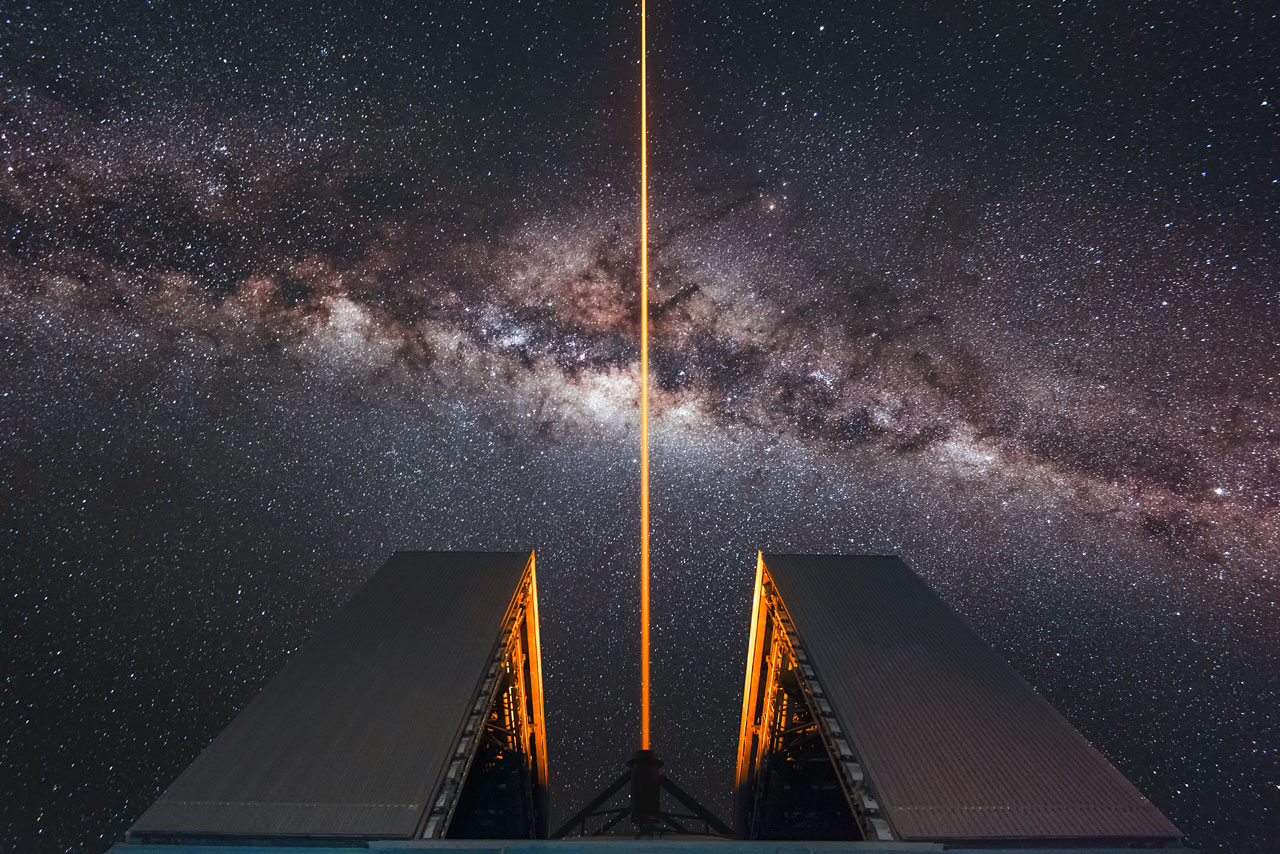
\includegraphics[width=0.9\linewidth]{Images/lgs2.jpg}
		%\end{minipage}
		%\begin{minipage}{.45\textwidth}
		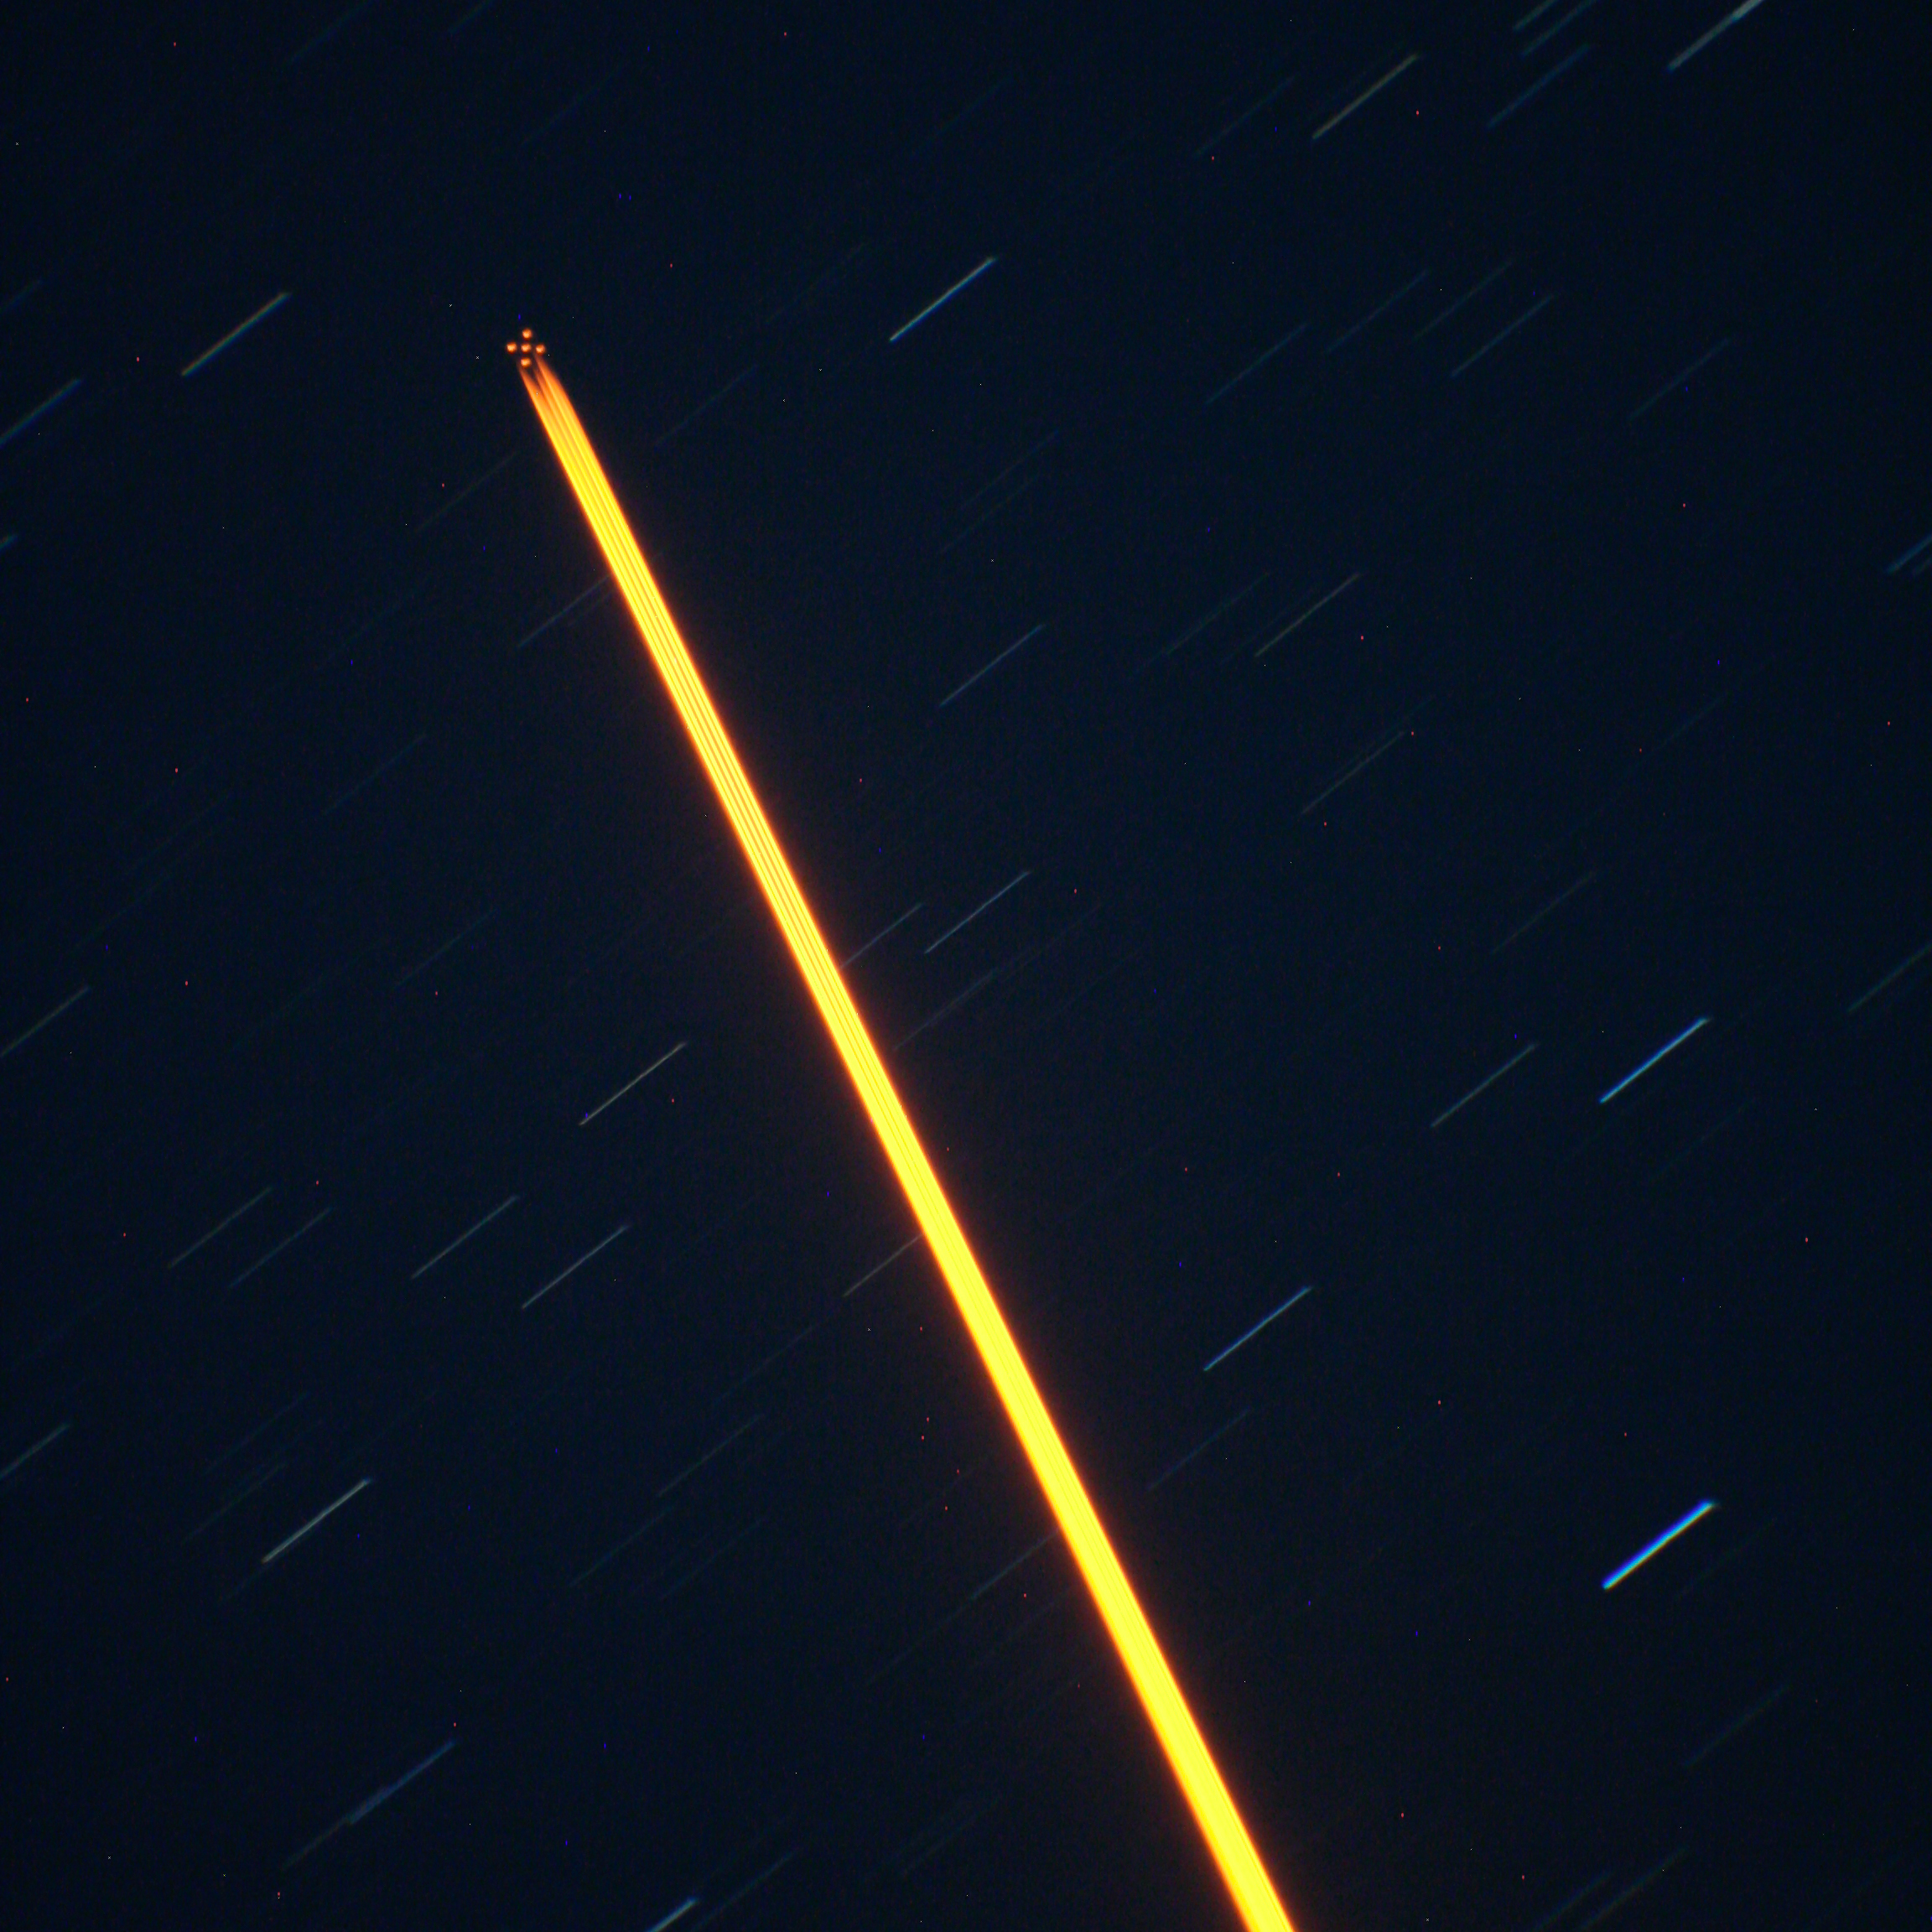
\includegraphics[width = .8\textwidth]{Images/lgsinsky.jpg}
		%\end{minipage}
		\caption{Long exposure of a laser guide star created by the Gemini Observatory as seen in the night sky \protect\cite{gemini}.}
		%\caption{Laser guide star shone into the night sky at ESO's Very Large Telescope \protect\cite{lgs2} (left) and a time lapse of a laser guide star as seen in the sky \protect\cite{gemini}.}
		\label{fig:lgs2}
\end{figure}

One important property of laser guide stars is their brightness, which can be increased by improving the intensity of the laser beam, increasing the size of the laser beam, or by using various optical techniques to increase the atom's probability of absorbing and emitting photons. Nevertheless, there remain ``the three evils'' of laser guide stars, each of which decreases brightness: Larmor precession, recoil, and transition saturation (i.e. depumping). Larmor precession, depicted in Fig. \ref{fig:larpre}, is the precession of the atom's total atomic angular momentum vector about the axis of the magnetic field. It arises in atoms that possess a magnetic moment, and thus experience a torque in a magnetic field. This phenomenon decreases the benefits obtained from optical pumping through a nonoptimal redistribution of the atom's angular momentum vector. The second ``evil,'' recoil, is due to the spontaneous emission of photons, which causes the atom to gain velocity in order to conserve momentum. Due to the Doppler effect, a redshift occurs, rendering the atom unable to absorb more laser light. The third ``evil,'' transition saturation, is the depopulation of atoms from a higher ground state to a lower ground state, resulting in a different wavelength for absorption \cite{Holzlohner2012}. We focus on mitigating the effects of Larmor precession, but will also briefly consider transition saturation.

\begin{figure}[h]
		\centering
		\begin{tikzpicture}
			\node at (0,0) {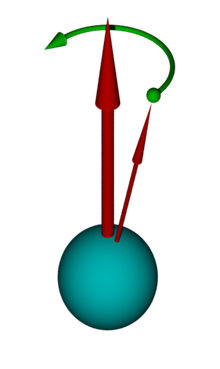
\includegraphics[scale = .5]{Images/larmorprecession.png}};
			\node at (1,1) {$\vec \mu$};
			\node at (0,3.5) {$\vec B$};
			\node at (1.5,2.5) {$\omega$};
		\end{tikzpicture}
		\caption{Schematic of an atom with an angular momentum vector $\vec \mu$ precessing about a magnetic field $\vec B$ with angular speed $\omega$ \protect\cite{larmor}.}
		\label{fig:larpre}
\end{figure}


In 2014, Kane et al. proposed a technique to improve laser guide stars, which they coined \textit{magnetic resonant pulsing} (MRP) \cite{Kane2014}. This technique proposes using a pulsed laser beam with a repetition rate equal to the atom's Larmor frequency, the frequency of the atom's precession in the magnetic field. For sodium in the Earth's magnetic field, these frequencies are typically around \SI{200}{\kilo Hz} to \SI{400}{\kilo Hz}. MRP has been computationally simulated by Rampy et al. and Kane et al. \cite{Rampy2010,Kane2014}. Their data show that lasers pulsed at the Larmor frequency of the atom in a magnetic field increase photon return when compared with continuous wave light as the direction of the laser beam nears perpendicular to the magnetic field.

In this thesis, we experimentally test MRP under controlled conditions. We build a laser with wavelength on resonance with rubidium and capable of being operated in continuous wave or pulsed mode using a diode laser chopped with an acousto-optic modulator (AOM). Although laser guide stars involve laser light interacting with sodium, we instead use rubidium since it is similar to sodium (including a similar gyromagnetic ratio, magnetic moment, and Larmor frequency, in addition to both being alkali metals), but because it is also the overall focus of this laboratory. Fluorescence measurements are taken of rubidium atoms confined in an absorption cell and surrounded by a variable magnetic field. 


Since the Larmor precession of an atom depends linearly on the strength of the magnetic field, we are able to change the frequency of the atom's precession to any frequency within the range of $\SI{200}{\kilo \hertz}$ to $\SI{2000}{\kilo \hertz}$ by changing the strength of the magnetic field. Thus, we can bring the system into and out of magnetic resonant pulsing by adjusting the strength of the magnetic field while measuring the amount of light the atoms absorb and emit. By changing the orientation of the magnetic fields with respect to the laser beam, we are able to test the dependence of fluorescence upon the angle between the magnetic field and the laser beam. 

In Chapter 2, we outline the atomic and quantum theory that underpins laser guide stars and the details of magnetic resonant pulsing. In Chapter 3, we detail the experimental laser system with wavelength on resonance with rubidium and pulsed at the Larmor frequency. Chapter 4 describes the magnetic field configuration used. In Chapter 5, we detail the final experimental setup, show how measurements were made, and present the results of the fluorescence measurements. Chapter 6 concludes this thesis, presents problems encountered, and provides an outlook for future experiments. Appendix A discusses laser guide stars in more detail and Appendix B introduces and describes the method of adaptive optics. Appendix C describes a proposed, nonfunctional dye laser that was built for this experiment but later abandoned. 


